These subsections are about inputs that carry an instruction.

\subsection{Five tasks with instructions: the certified switch}
\label{sec:five}

Five tasks, T5-base, 10 epochs per task, \FiveCertSeeds{} seeds; the answers are re-tested against all reference answers. The following holds for every test in this paper unless a test says otherwise. It is a reduced setting: a tenth of the published budget, a smaller model, and one step of the published methods (a singular value decomposition that the official code delegates to a library that did not load on the free GPUs) computed with PyTorch without a check that the two agree number for number (Appendix~\ref{app:impl}). The five tasks are among the 15 tasks of Section~\ref{sec:fifteen}. The rewordings of the definitions were written by machine during development and looked at during the design (``development rewordings''); they are not rewordings by people. Tests marked ``routes only'' compute where inputs go and train nothing. Statements about InfLoRA and GainLoRA hold only for this setting.

\begin{table}[t]
  \caption{Five-task sequence, original instructions. Score right after learning: average score of each task right after it was learned. AP: average score after the last task. Answers changed: test inputs of the first four
  tasks whose answer at the end differs from the answer right after their task was learned.
  Certified: test inputs inside a zone.
  Scores are means over \FiveCertSeeds{} seeds, with the lowest and the highest seed in brackets; counts are summed over the seeds.}
  \label{tab:fivemain}
  \centering
  \small
  \setlength{\tabcolsep}{4pt}
  \begin{tabular}{lccccc}
    \toprule
    Method & \shortstack[c]{Score\\right after\\learning $\uparrow$} & \shortstack[c]{Final\\score $\uparrow$} & \shortstack[c]{Forgetting\\(points) $\downarrow$} & \shortstack[c]{Answers\\changed $\downarrow$} & Certified inputs \\
    \midrule
    \cert{} (ours) & 79.74 {\scriptsize(79.2--80.8)} & 79.74 {\scriptsize(79.2--80.8)} & 0.00 & 0 of 1{,}200 & 1{,}500 of 1{,}500 \\
    \nearest{} & 79.74 {\scriptsize(79.2--80.8)} & 79.74 {\scriptsize(79.2--80.8)} & 0.00 & 0 of 1{,}200 &  \\
    \centre{} & 79.74 {\scriptsize(79.2--80.8)} & 79.74 {\scriptsize(79.2--80.8)} & 0.00 & 0 of 1{,}200 &  \\
    \keyswitch{} & 79.74 {\scriptsize(79.2--80.8)} & 79.74 {\scriptsize(79.2--80.8)} & 0.00 & 0 of 1{,}200 &  \\
    \plain{} & 79.74 {\scriptsize(79.2--80.8)} & 36.08 {\scriptsize(32.3--39.5)} & 54.58 {\scriptsize(51.6--58.6)} & 994 of 1{,}200 &  \\
    \midrule
    InfLoRA & 60.02 {\scriptsize(56.6--63.3)} & 62.93 {\scriptsize(59.0--65.4)} & $-$3.14 {\scriptsize($-$5.3 to $-$1.7)} & 370 of 1{,}200 &  \\
    GainLoRA & 61.42 {\scriptsize(59.1--64.4)} & 61.96 {\scriptsize(60.9--63.9)} & $-$0.51 {\scriptsize($-$2.6 to 0.7)} & 65 of 1{,}200 &  \\
    \bottomrule
\end{tabular}

\end{table}

\begin{figure}[t]
  \centering
  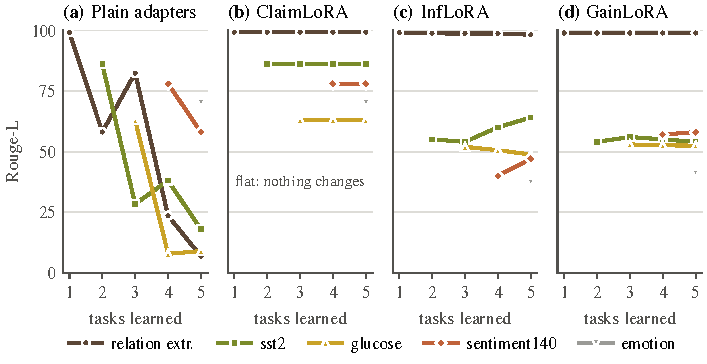
\includegraphics[width=\linewidth]{figures/five_tracks}
  \caption{Score of each of the five tasks as further tasks are learned (seed 42, original
  instructions). Plain adapters fall as soon as the next task is learned; the certified
  switch gives flat lines; the two published methods are flat at a lower level.}
  \label{fig:fivetracks}
\end{figure}

\paragraph{The certified switch keeps every answer.} After the fifth task its average score equals the
score right after learning, \FiveCertAP{} Rouge-L; forgetting is \FiveCertFT{}, and none of
the \FiveCertCompared{} answers to the test inputs of the first four tasks changed. All \FiveCertInputsOne{} test inputs lie inside
their own zone (Proposition~\ref{prop:own}), and no training input of a later
task lay inside an older zone (\FiveCertBlocked{} of \FiveCertTrainInputs{}). This is what Theorem~\ref{thm:writeonce} says; the run confirms that the implementation does what the theorem describes. With the original instructions
\nearest{}, \centre{} and \keyswitch{} choose the same routes and give the same numbers.

\paragraph{The same adapters without a switch lose most of what they learned.} With all adapters on (\plain{}), the average falls to
\FivePlainAP{}, forgetting is \FivePlainFT{} points, and most of the
\FivePlainCompared{} answers change. Only the task learned last is intact.

\paragraph{The published methods learned less here.} InfLoRA and GainLoRA have forgetting scores near zero (\FiveInfFT{} points for InfLoRA; a
negative value means that old tasks improved on average), though \FiveInfChanged{} of \FiveInfCompared{} answers of InfLoRA and \FiveGainChanged{} of \FiveGainCompared{} of GainLoRA change; changes for the better and for the worse cancel in the score. They end at \FiveInfAP{} (InfLoRA),
well below the certified switch, because they are lower from the start: right
after learning they stand at \FiveInfLearned{} and \FiveGainLearned{}, against
\FivePlainLearned{} for plain adapters (Table~\ref{tab:fivemain}). Both learn relation extraction but not the classification tasks within ten epochs; on SST-2 and Sentiment140 they are at the level of guessing right after learning (Table~\ref{tab:instdetail}). \textbf{So in our runs these two methods were at the level of guessing on two of the five tasks and clearly below plain adapters on a third, and the comparison cannot show how well they retain what they learn.} We do not know how much of this is the method and how much is our set-up.

\paragraph{Official script, and the same seed twice.} The scores of the official script (one randomly picked reference per input) lead to the same reading as the re-test (Table~\ref{tab:fiveofficial}; agreement of the answers in Table~\ref{tab:instdetail}). Seed 42 was run twice in separate sessions on the same kind of GPU: the first task was reproduced answer for answer (for \cert{} and InfLoRA also the second), the later ones were not, so training is not reproducible bit for bit and differences of a few tenths of a point mean nothing. The count for the certified switch does not vary: no answer of an earlier task changed in either run, nor in any other seed. The tables use the second run, made together with seeds 43 and 44.

\subsection{Reworded instructions}
\label{sec:reworded}

\begin{table}[t]
  \caption{Five tasks with the original and with three levels of rewording: average score at the end and
  number of changed answers. The adapters are those of Table~\ref{tab:fivemain}; nothing is
  retrained. Means and sums over the seeds.}
  \label{tab:fivewordings}
  \centering
  \small
  \setlength{\tabcolsep}{4.5pt}
  \begin{tabular}{lcccccccc}
    \toprule
    & \multicolumn{4}{c}{Final score $\uparrow$} & \multicolumn{4}{c}{Answers changed (of 1{,}200) $\downarrow$} \\
    \cmidrule(lr){2-5} \cmidrule(lr){6-9}
    Method & original & light & medium & heavy & original & light & medium & heavy \\
    \midrule
    \cert{} (ours) & 79.7 & 79.6 & 79.0 & 74.1 & 0 & 0 & 0 & 0 \\
    \nearest{} & 79.7 & 79.6 & 79.0 & 74.1 & 0 & 0 & 0 & 0 \\
    \centre{} & 79.7 & 79.6 & 78.4 & 59.4 & 0 & 0 & 0 & 171 \\
    \keyswitch{} & 79.7 & 36.4 & 36.0 & 35.2 & 0 & 985 & 1{,}001 & 939 \\
    \plain{} & 36.1 & 36.4 & 36.0 & 35.2 & 994 & 985 & 1{,}001 & 939 \\
    \midrule
    InfLoRA & 62.9 & 64.3 & 57.8 & 54.3 & 370 & 296 & 320 & 470 \\
    GainLoRA & 62.0 & 64.6 & 58.8 & 51.6 & 65 & 58 & 122 & 178 \\
    \bottomrule
\end{tabular}

\end{table}

\begin{figure}[t]
  \centering
  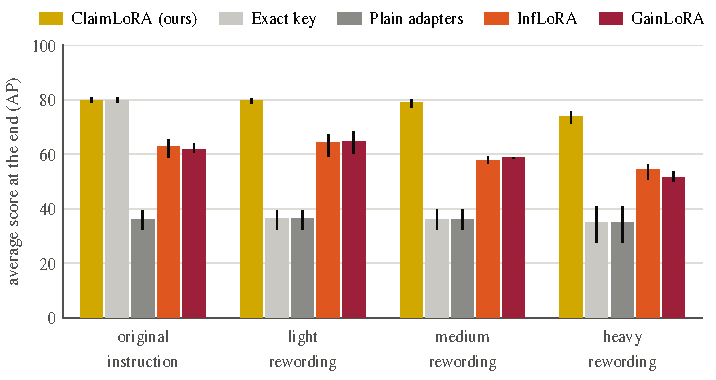
\includegraphics[width=0.9\linewidth]{figures/five_wordings}
  \caption{Average score at the end (AP) on the five tasks, original instructions and
  three levels of rewording. Bars are means over seeds; a black line spans the lowest and the highest seed.}
  \label{fig:fivewordings}
\end{figure}

\begin{table}[t]
  \caption{Routes on the five tasks: test inputs that are certified, given to
  their own task, and whose answers change, for the certified switch and for the nearest-centre
  rule. Routes do not depend on the seed; counts are summed over seeds.}
  \label{tab:fiveroutes}
  \centering
  \small
  \setlength{\tabcolsep}{4.5pt}
  \begin{tabular}{lcccccc}
    \toprule
    & & \multicolumn{3}{c}{\cert{}} & \multicolumn{2}{c}{\centre{}} \\
    \cmidrule(lr){3-5} \cmidrule(lr){6-7}
    Wording & Tasks & Certified inputs & \shortstack[c]{Sent to own\\task $\uparrow$} & \shortstack[c]{Answers\\changed $\downarrow$} & \shortstack[c]{Sent to own\\task $\uparrow$} & \shortstack[c]{Answers\\changed $\downarrow$} \\
    \midrule
    original & 5 & 1{,}500 of 1{,}500 & 100.0\% & 0 of 1{,}200 & 100.0\% & 0 of 1{,}200 \\
    light & 5 & 1{,}500 of 1{,}500 & 100.0\% & 0 of 1{,}200 & 100.0\% & 0 of 1{,}200 \\
    medium & 5 & 300 of 1{,}500 & 100.0\% & 0 of 1{,}200 & 99.2\% & 0 of 1{,}200 \\
    heavy & 5 & 294 of 1{,}500 & 93.8\% & 0 of 1{,}200 & 72.2\% & 171 of 1{,}200 \\
    \bottomrule
\end{tabular}

\end{table}

A benchmark input carries its task definition word for word, so any rule that recognises the
definition looks perfect. The test that separates the rules asks the same task in other
words: the evaluation is repeated with the light, medium and heavy rewording of each definition.

\paragraph{No answer changes under any wording.} For the certified switch the count of changed answers is zero in every column. For the light rewording this is guaranteed, because all \FiveCertZoneOneLight{} inputs are
still certified. For the medium and the heavy rewording it is not: only \FiveCertZoneOneMedium{} and \FiveCertZoneOneHeavy{} of the \FiveCertInputsOne{}
inputs are inside a zone, all of relation extraction, the task with the longest instruction. The others kept their answers because no later task came nearer to them than
their own, which Proposition~\ref{prop:uncertified} permits but does not
promise; in an order where SST-2 is learned after
Sentiment140, 31 routes of heavily reworded inputs would change (Section~\ref{sec:orders}). The average
score falls from \FiveCertAP{} to \FiveCertAPHeavy{} at the heavy wording (Table~\ref{tab:fivewordings}, Figure~\ref{fig:fivewordings}).

\paragraph{Other rules.} \keyswitch{} compares the opening token for token: with the light rewording it recognises nothing, leaves
all adapters on and ends where \plain{} ends. \nearest{} and \cert{} score alike on this benchmark; the radius decides which inputs also carry the guarantee. \centre{}, the nearest-centre rule with the token weights of Eq.~\eqref{eq:weights}, gives only
\FiveCentreRightHeavy{}\% of the heavily reworded inputs to their own task, scores far below \cert{} and
changes answers as later tasks arrive (Tables~\ref{tab:fivewordings}, \ref{tab:fiveroutes}; \FiveCentreComparedHeavy{} answers compared). The first version of \cert{}, the nearest centre
with all tokens weighted equally, did better here (97.4\% to the right task with seed 42, against
\FiveCertRightHeavy{}\% for the final rule) and was replaced because it failed on the 15-task sequence (Appendix~\ref{app:history}). The published methods have no recognition step that a rewording could break; their forgetting scores stay within a few points in every wording, and the most answers differ under heavy rewording (Table~\ref{tab:fivewordings}, of \FiveInfComparedHeavy{}).

\paragraph{Where the loss under heavy rewording comes from.} None of the drop from \FiveCertAP{} to \FiveCertAPHeavy{} is forgetting. One part is that the adapters answer
a reworded instruction less well: with all adapters on, right after each task, the score is
\FivePlainLearnedHeavy{}. The other part is routing:
\FiveCertWrongHeavy{} of the \FiveCertInputsOne{} heavily reworded inputs go to another task,
which brings \FivePlainLearnedHeavy{} down to the final \FiveCertAPHeavy{}. All of them are tweets of
Sentiment140 given to SST-2, the other sentiment task.

\begin{figure}[t]
  \centering
  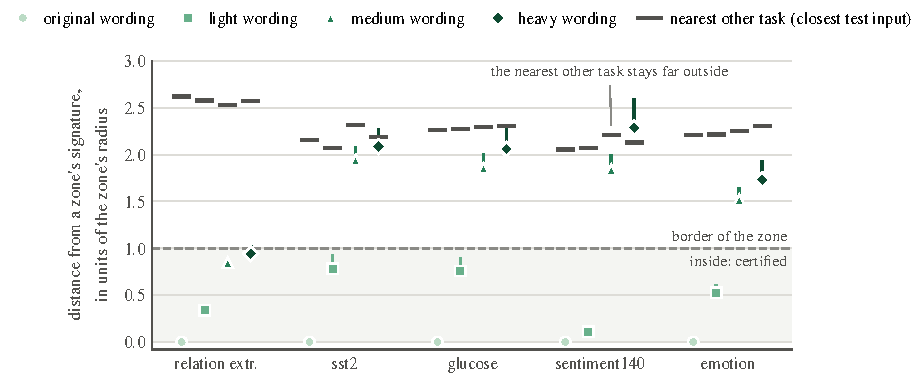
\includegraphics[width=0.92\linewidth]{figures/margins}
  \caption{Why rewording costs the certificate before it costs the route (five tasks, T5-base
  word-vectors). Markers: relative distance $\delta_k$ of the test inputs of a task from their own
  signature, in units of the radius of their own zone: median over the 100 inputs, with a line up to
  the farthest input. Short dark lines: how close the closest of these inputs comes to the signature of any
  \emph{other} task, in units of that task's radius. Below the dashed line an input is inside the
  zone, that is, certified.}
  \label{fig:margins}
\end{figure}

\paragraph{Where reworded inputs lie.}\label{sec:geometry} With the original
wording every input lies exactly on the signature of its task (Proposition~\ref{prop:own}). The
light rewordings move inputs by 0.1 to 0.8 radii, inside the zone. The medium and heavy
rewordings move them by 1.5 to 2.3 radii in four of the five tasks, outside; relation
extraction stays inside. The signatures of the other tasks are 2.1 to 2.6 of \emph{their} radii away, so an input that has left its
zone is mostly still nearer to its own signature than to any other: the
certificate is lost long before the route. The margins cross where the errors are: under heavy rewording the tweets of Sentiment140 lie 2.29 radii from their
own signature (up to 2.60), and the signature of SST-2 is 2.13 of its
radii from the closest of them (Appendix~\ref{app:more}, Table~\ref{tab:geometry}).

\subsection{Routes from the example alone: rewording cannot change the route}
\label{sec:exampleroutes}

Under heavy rewording \cert{} sends some inputs to another task (Section~\ref{sec:reworded}), while \recog{} never
reads the instruction (Remark~\ref{rem:auditlimits}(v)). The five tasks were trained once more
with their definitions (plain adapters, nothing blocked); \recog{} and
\handicap{} route from the example alone, with the route table of the runs without
instructions (Section~\ref{sec:nodeftrained}). The scores of \cert{} equal those of the single-seed run of seed 42 with definitions, not those of the three-seed run of Table~\ref{tab:fivewordings} (seed 42 was trained twice; Section~\ref{sec:five}).

\begin{table}[t]
  \caption{The five tasks with their definitions, seed 42, plain adapters; the
  same adapters under each rule, at the four wordings. Top: final score (AP).
  Bottom: answers of the first four tasks that differ at the end, of \AudUCompared{}. ``Zone first'': the certified route where the input is
  inside a zone, otherwise the route of \recog{} or \handicap{}. The rows of the published
  methods are from Section~\ref{sec:reworded}.}
  \label{tab:instanceroutes}
  \centering
  {\scriptsize\setlength{\tabcolsep}{2pt}\begin{tabular}{p{1.2in}rrrrrrrrr}
    \toprule
    & \multicolumn{4}{c}{Final score $\uparrow$} & \multicolumn{4}{c}{\shortstack{Answers changed\\of \AudUCompared{} $\downarrow$}} & \shortstack[r]{Sent to own\\task, heavy, \% $\uparrow$} \\
    \cmidrule(lr){2-5}\cmidrule(lr){6-9}
    & original & light & medium & heavy & original & light & medium & heavy & \\
    \midrule
    \cert{} (zones on the instruction) & \AudUOriginalCertAP{} & \AudULightCertAP{} & \AudUMediumCertAP{} & \AudUHeavyCertAP{} & \AudUOriginalCertChanged{} & \AudULightCertChanged{} & \AudUMediumCertChanged{} & \AudUHeavyCertChanged{} & \AudUHeavyCertRight{} \\
    \recog{} (example alone) & \AudUOriginalRidgeAP{} & \AudULightRidgeAP{} & \AudUMediumRidgeAP{} & \AudUHeavyRidgeAP{} & \AudUOriginalRidgeChanged{} & \AudULightRidgeChanged{} & \AudUMediumRidgeChanged{} & \AudUHeavyRidgeChanged{} & \AudUHeavyRidgeRight{} \\
    \handicap{}, $\nu = 2$ (example alone) & \AudUOriginalHandicapAP{} & \AudULightHandicapAP{} & \AudUMediumHandicapAP{} & \AudUHeavyHandicapAP{} & \AudUOriginalHandicapChanged{} & \AudULightHandicapChanged{} & \AudUMediumHandicapChanged{} & \AudUHeavyHandicapChanged{} & \AudUHeavyHandicapRight{} \\
    every input to its own task (ceiling) & \AudUOriginalOwnAP{} & \AudULightOwnAP{} & \AudUMediumOwnAP{} & \AudUHeavyOwnAP{} & \AudUOriginalOwnChanged{} & \AudULightOwnChanged{} & \AudUMediumOwnChanged{} & \AudUHeavyOwnChanged{} & \AudUHeavyOwnRight{} \\
    zone first, else \recog{} & \AudUOriginalMixRidgeAP{} & \AudULightMixRidgeAP{} & \AudUMediumMixRidgeAP{} & \AudUHeavyMixRidgeAP{} & \AudUOriginalMixRidgeChanged{} & \AudULightMixRidgeChanged{} & \AudUMediumMixRidgeChanged{} & \AudUHeavyMixRidgeChanged{} & \AudUHeavyMixRidgeRight{} \\
    zone first, else \handicap{} & \AudUOriginalMixHandicapAP{} & \AudULightMixHandicapAP{} & \AudUMediumMixHandicapAP{} & \AudUHeavyMixHandicapAP{} & \AudUOriginalMixHandicapChanged{} & \AudULightMixHandicapChanged{} & \AudUMediumMixHandicapChanged{} & \AudUHeavyMixHandicapChanged{} & \AudUHeavyMixHandicapRight{} \\
    \centre{} & \AudUOriginalCentreAP{} & \AudULightCentreAP{} & \AudUMediumCentreAP{} & \AudUHeavyCentreAP{} & \AudUOriginalCentreChanged{} & \AudULightCentreChanged{} & \AudUMediumCentreChanged{} & \AudUHeavyCentreChanged{} & \AudUHeavyCentreRight{} \\
    \plain{} & \AudUOriginalPlainAP{} & \AudULightPlainAP{} & \AudUMediumPlainAP{} & \AudUHeavyPlainAP{} & \AudUOriginalPlainChanged{} & \AudULightPlainChanged{} & \AudUMediumPlainChanged{} & \AudUHeavyPlainChanged{} & \AudUHeavyPlainRight{} \\
    \midrule
    GainLoRA & \AudWordOriginalGainloraAP{} & \AudWordLightGainloraAP{} & \AudWordMediumGainloraAP{} & \AudWordHeavyGainloraAP{} & \AudWordOriginalGainloraChanged{} & \AudWordLightGainloraChanged{} & \AudWordMediumGainloraChanged{} & \AudWordHeavyGainloraChanged{} & -- \\
    InfLoRA & \AudWordOriginalInfloraAP{} & \AudWordLightInfloraAP{} & \AudWordMediumInfloraAP{} & \AudWordHeavyInfloraAP{} & \AudWordOriginalInfloraChanged{} & \AudWordLightInfloraChanged{} & \AudWordMediumInfloraChanged{} & \AudWordHeavyInfloraChanged{} & -- \\
    \bottomrule
\end{tabular}}

\end{table}

\paragraph{Seed 42.} Line fixed before the run: \recog{} ``repairs the weak spot'' if its final score at the heavy
wording is at least 2 points above that of \cert{}, its score at the original wording is within
2 points of \cert{}, and at most 8 of the \AudUCompared{} compared answers change at every wording;
it ``does not'' if the heavy score is below that of \cert{} or the original score more than 4
points below. Verdict: all three lines hold (Table~\ref{tab:instanceroutes}). At the heavy wording \recog{} ends at
\AudUHeavyRidgeAP{}, and \handicap{} close to it, above \cert{}; the ceiling, with every input at its own task, is \AudUHeavyOwnAP{}. Our guesses (78.5 to 79.3 at the original wording, 75.5 to 76.7 at the heavy one) held. One was wrong in the good direction: we expected about six changed answers for \recog{}, as without definitions; six routes change, but for three
of these inputs the model gives the same answer with the adapters up to either task, and why fewer answers change with the definition we did not test. The routes of \recog{} are the same at every wording, so it stays
\AudURidgeBelowOwnLow{} to \AudURidgeBelowOwnHigh{} points below the ceiling (\handicap{}: \AudUHandicapBelowOwnLow{} to \AudUHandicapBelowOwnHigh{}): what is lost
under rewording is what the adapters themselves lose, not misrouting, while \cert{} loses
\AudUHeavyCertBelowOwn{} points at the heavy wording through misrouted
inputs. The mixed rule is best at the original, light and heavy wording and below \cert{} at the medium one, whose own fallback is right for every input there.

\paragraph{Three seeds.} An independent reading pointed out that seed 42 is the seed in which \cert{} loses most at the heavy wording, so seeds 43 and 44 were added (Table~\ref{tab:instanceroutesseeds}).
Line fixed before these runs, for the means over the three seeds: the result ``stands for three seeds'' if the heavy score of \recog{} is at least 2 points above that of \cert{}, the original score is within 2 points of \cert{}, and in every seed at most 8 of \AudUCompared{} answers change at every wording.
Verdict: it stands. At the heavy wording \recog{} ends at \AudUThreeHeavyRidgeAP{}, a gain of \AudUThreeHeavyRidgeAboveCert{} points over \cert{}; at the original wording it is \AudUThreeOriginalRidgeBelowCert{} points below \cert{}; in no seed and at no wording do more than \AudUThreeMaxChangedPerSeed{} answers change under \recog{}. Over the four wordings \recog{} stays \AudUThreeRidgeBelowOwnLow{} to \AudUThreeRidgeBelowOwnHigh{} points below the ceiling and \handicap{} \AudUThreeHandicapBelowOwnLow{} to \AudUThreeHandicapBelowOwnHigh{}; \cert{} loses \AudUThreeHeavyCertBelowOwn{} points at the heavy wording.
We had expected a smaller gain, 2 to 2.5 points: in seeds 43 and 44 the adapters lose less under heavy rewording than in seed 42.
These three seeds are not the training runs of Table~\ref{tab:fivewordings}: seed 42 is the single-seed run, and seeds 43 and 44 were trained again. So \cert{} ends at \AudUThreeOriginalCertAPOne{} (original) and \AudUThreeHeavyCertAPOne{} (heavy) here, and at \FiveCertAP{} and \FiveCertAPHeavy{} in Table~\ref{tab:fivewordings}; the difference is of the size seen between two runs of the same seed.
It remains five tasks, with three development rewordings per task, not rewordings by people; Remark~\ref{rem:auditlimits}(v) says what this assumes about the input.

\begin{table}[t]
  \caption{As Table~\ref{tab:instanceroutes}, means over \AudUThreeSeeds{} seeds (42, 43, 44); changed answers are summed over the seeds. Training runs: seed 42 as in Table~\ref{tab:instanceroutes}, seeds 43 and 44 trained for this table; they are not the runs of Table~\ref{tab:fivewordings}, so the rows of \cert{} differ from it by a few tenths of a point.}
  \label{tab:instanceroutesseeds}
  \centering
  {\scriptsize\setlength{\tabcolsep}{2pt}\begin{tabular}{p{1.2in}rrrrrrrrr}
    \toprule
    & \multicolumn{4}{c}{Final score $\uparrow$} & \multicolumn{4}{c}{\shortstack{Answers changed\\of \AudUThreeCompared{} $\downarrow$}} & \shortstack[r]{Sent to own\\task, heavy, \% $\uparrow$} \\
    \cmidrule(lr){2-5}\cmidrule(lr){6-9}
    & original & light & medium & heavy & original & light & medium & heavy & \\
    \midrule
    \cert{} (zones on the instruction) & \AudUThreeOriginalCertAP{} & \AudUThreeLightCertAP{} & \AudUThreeMediumCertAP{} & \AudUThreeHeavyCertAP{} & \AudUThreeOriginalCertChanged{} & \AudUThreeLightCertChanged{} & \AudUThreeMediumCertChanged{} & \AudUThreeHeavyCertChanged{} & \AudUThreeHeavyCertRight{} \\
    \recog{} (example alone) & \AudUThreeOriginalRidgeAP{} & \AudUThreeLightRidgeAP{} & \AudUThreeMediumRidgeAP{} & \AudUThreeHeavyRidgeAP{} & \AudUThreeOriginalRidgeChanged{} & \AudUThreeLightRidgeChanged{} & \AudUThreeMediumRidgeChanged{} & \AudUThreeHeavyRidgeChanged{} & \AudUThreeHeavyRidgeRight{} \\
    \handicap{}, $\nu = 2$ (example alone) & \AudUThreeOriginalHandicapAP{} & \AudUThreeLightHandicapAP{} & \AudUThreeMediumHandicapAP{} & \AudUThreeHeavyHandicapAP{} & \AudUThreeOriginalHandicapChanged{} & \AudUThreeLightHandicapChanged{} & \AudUThreeMediumHandicapChanged{} & \AudUThreeHeavyHandicapChanged{} & \AudUThreeHeavyHandicapRight{} \\
    every input to its own task (ceiling) & \AudUThreeOriginalOwnAP{} & \AudUThreeLightOwnAP{} & \AudUThreeMediumOwnAP{} & \AudUThreeHeavyOwnAP{} & \AudUThreeOriginalOwnChanged{} & \AudUThreeLightOwnChanged{} & \AudUThreeMediumOwnChanged{} & \AudUThreeHeavyOwnChanged{} & \AudUThreeHeavyOwnRight{} \\
    zone first, else \recog{} & \AudUThreeOriginalMixRidgeAP{} & \AudUThreeLightMixRidgeAP{} & \AudUThreeMediumMixRidgeAP{} & \AudUThreeHeavyMixRidgeAP{} & \AudUThreeOriginalMixRidgeChanged{} & \AudUThreeLightMixRidgeChanged{} & \AudUThreeMediumMixRidgeChanged{} & \AudUThreeHeavyMixRidgeChanged{} & \AudUThreeHeavyMixRidgeRight{} \\
    zone first, else \handicap{} & \AudUThreeOriginalMixHandicapAP{} & \AudUThreeLightMixHandicapAP{} & \AudUThreeMediumMixHandicapAP{} & \AudUThreeHeavyMixHandicapAP{} & \AudUThreeOriginalMixHandicapChanged{} & \AudUThreeLightMixHandicapChanged{} & \AudUThreeMediumMixHandicapChanged{} & \AudUThreeHeavyMixHandicapChanged{} & \AudUThreeHeavyMixHandicapRight{} \\
    \centre{} & \AudUThreeOriginalCentreAP{} & \AudUThreeLightCentreAP{} & \AudUThreeMediumCentreAP{} & \AudUThreeHeavyCentreAP{} & \AudUThreeOriginalCentreChanged{} & \AudUThreeLightCentreChanged{} & \AudUThreeMediumCentreChanged{} & \AudUThreeHeavyCentreChanged{} & \AudUThreeHeavyCentreRight{} \\
    \plain{} & \AudUThreeOriginalPlainAP{} & \AudUThreeLightPlainAP{} & \AudUThreeMediumPlainAP{} & \AudUThreeHeavyPlainAP{} & \AudUThreeOriginalPlainChanged{} & \AudUThreeLightPlainChanged{} & \AudUThreeMediumPlainChanged{} & \AudUThreeHeavyPlainChanged{} & \AudUThreeHeavyPlainRight{} \\
    \midrule
    GainLoRA & \AudUThreeOriginalGainloraAP{} & \AudUThreeLightGainloraAP{} & \AudUThreeMediumGainloraAP{} & \AudUThreeHeavyGainloraAP{} & \AudUThreeOriginalGainloraChanged{} & \AudUThreeLightGainloraChanged{} & \AudUThreeMediumGainloraChanged{} & \AudUThreeHeavyGainloraChanged{} & -- \\
    InfLoRA & \AudUThreeOriginalInfloraAP{} & \AudUThreeLightInfloraAP{} & \AudUThreeMediumInfloraAP{} & \AudUThreeHeavyInfloraAP{} & \AudUThreeOriginalInfloraChanged{} & \AudUThreeLightInfloraChanged{} & \AudUThreeMediumInfloraChanged{} & \AudUThreeHeavyInfloraChanged{} & -- \\
    \bottomrule
\end{tabular}}

\end{table}

\subsection{Fifteen tasks with instructions}
\label{sec:fifteen}

The five-task sequence was chosen by us. To test a sequence we did not choose, the 15 tasks of the official order~1 of Super-NaturalInstructions were run with the same
model, budget and code, for the certified switch and the two published methods: one seed, 3.1 to 3.5 hours per run on a free GPU.

\begin{table}[t]
  \caption{Fifteen-task sequence, original instructions (seed 42; columns as in Table~\ref{tab:fivemain}). ``Changed'' counts
  test inputs of the first 14 tasks.}
  \label{tab:fifteenmain}
  \centering
  \small
  \setlength{\tabcolsep}{4pt}
  \begin{tabular}{lccccc}
    \toprule
    Method & \shortstack[c]{Score\\right after\\learning $\uparrow$} & \shortstack[c]{Final\\score $\uparrow$} & \shortstack[c]{Forgetting\\(points) $\downarrow$} & \shortstack[c]{Answers\\changed $\downarrow$} & Certified inputs \\
    \midrule
    \cert{} (ours) & 42.77 & 42.77 & 0.00 & 0 of 1{,}097 & 1{,}197 of 1{,}197 \\
    \nearest{} & 42.77 & 42.77 & 0.00 & 0 of 1{,}097 &  \\
    \centre{} & 42.77 & 42.63 & 0.15 & 2 of 1{,}097 &  \\
    \keyswitch{} & 42.77 & 42.77 & 0.00 & 0 of 1{,}097 &  \\
    \plain{} & 42.77 & 14.88 & 30.67 & 973 of 1{,}097 &  \\
    \midrule
    InfLoRA & 30.46 & 26.13 & 5.69 & 661 of 1{,}097 &  \\
    GainLoRA & 29.08 & 28.62 & 1.09 & 215 of 1{,}097 &  \\
    \bottomrule
\end{tabular}

\end{table}

\begin{figure}[t]
  \centering
  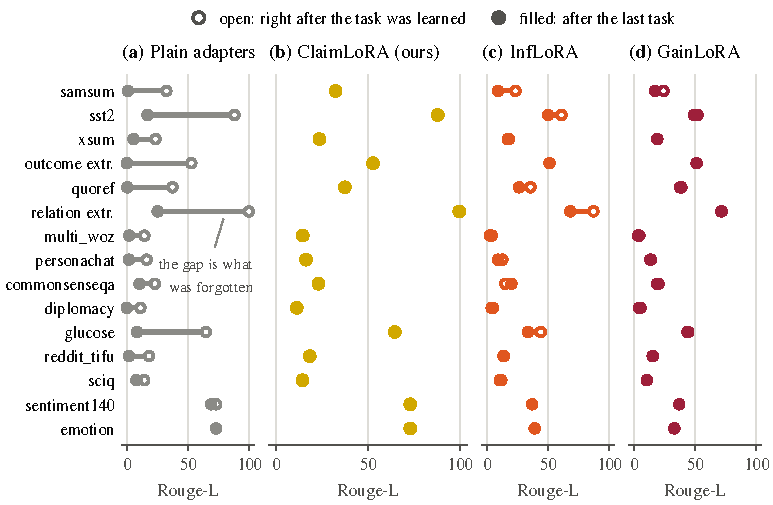
\includegraphics[width=\linewidth]{figures/fifteen_tasks}
  \caption{Score of each of the 15 tasks for four methods. Open circle: right after the task was
  learned. Filled circle: after the last task. For the
  certified switch the two circles coincide for every task.}
  \label{fig:fifteentasks}
\end{figure}

\paragraph{The certified switch keeps every answer.} Its average score after the 15th task equals
the score right after learning, \FifteenCertAP{} Rouge-L; forgetting is \FifteenCertFT{},
and none of the \FifteenCertCompared{} answers of the first 14 tasks changed. All \FifteenCertInputsOne{} test inputs lie
inside their own zone and no training input of a later task lay inside an older zone
(\FifteenCertBlocked{} of \FifteenCertTrainInputs{}), as Theorem~\ref{thm:writeonce}
guarantees. \nearest{} and \keyswitch{} give the same numbers, so
simpler rules reach the same score on this benchmark; \centre{} changes \FifteenCentreChanged{}
answers. With all adapters on the average falls to \FifteenPlainAP{} (forgetting \FifteenPlainFT{} points; most of \FifteenPlainCompared{} answers change), and every task except the last falls (Table~\ref{tab:fifteenpertask}).

\paragraph{The published methods learned less, and on fifteen tasks they also forget.} InfLoRA and
GainLoRA end at \FifteenInfAP{} and \FifteenGainAP{}. On five tasks
neither forgot; here InfLoRA forgets \FifteenInfFT{} points and GainLoRA \FifteenGainFT{}, and
\FifteenInfChanged{} (InfLoRA) and \FifteenGainChanged{} (GainLoRA) of \FifteenInfCompared{} answers differ at the end (Table~\ref{tab:fifteenmain}). The forgetting of InfLoRA is not
spread evenly (relation extraction, SST-2, SAMSum and Glucose fall most; Table~\ref{tab:instdetail}). Both
methods also learned less right after each task, \FifteenInfLearned{} and \FifteenGainLearned{}, against
\FifteenPlainLearned{} for plain adapters, so the gap to the
certified switch has two parts, a gap in learning and a smaller gap from forgetting (Section~\ref{sec:gap}). The official-script scores of InfLoRA are identical to those of an earlier run of the same method on Google Colab with the same seed (unlike the two five-task runs of seed 42, \fivefull{}).

\paragraph{The official script shows forgetting where no answer changed.} The official script gives
the certified switch an AP of \FifteenCertOffAP{} and a forgetting of \FifteenCertOffFT{}
(Table~\ref{tab:fifteenofficial}), although no answer changes. This is evaluation noise: the script scores each answer against one reference picked at random
on every load, and the re-test, which scores against all references, finds that none of the answers changed (agreement in Table~\ref{tab:instdetail}). When the claim is that nothing changed, the answers have to be
compared and not the scores. The official scores of InfLoRA and GainLoRA (AP \FifteenInfOffAP{} and \FifteenGainOffAP{}) lead to the same reading as
the re-test.

\begin{table}[t]
  \caption{Fifteen-task sequence with the original and with reworded instructions. The five tasks
  with rewordings sit inside the 15-task sequence. AP is the average score of these five tasks after the last task; ``Answers changed'' counts
  test inputs of the first four of them (of 400), and in the column ``original'' those of the first 14 tasks of the whole sequence (of 1{,}097). The adapters are those of Table~\ref{tab:fifteenmain};
  nothing is retrained.}
  \label{tab:fifteenwordings}
  \centering
  \small
  \setlength{\tabcolsep}{3.5pt}
  \begin{tabular}{lcccccccc}
    \toprule
    & \multicolumn{4}{c}{Final score $\uparrow$} & \multicolumn{4}{c}{Answers changed $\downarrow$} \\
    \cmidrule(lr){2-5} \cmidrule(lr){6-9}
    Method & original & light & medium & heavy & original & light & medium & heavy \\
    \midrule
    \cert{} (ours) & 42.8 & 80.7 & 80.2 & 76.0 & 0 & 0 & 0 & 0 \\
    \nearest{} & 42.8 & 80.7 & 80.2 & 76.0 & 0 & 0 & 0 & 0 \\
    \centre{} & 42.6 & 80.7 & 72.0 & 57.5 & 2 & 0 & 29 & 100 \\
    \keyswitch{} & 42.8 & 39.6 & 40.4 & 36.1 & 0 & 316 & 313 & 310 \\
    \plain{} & 14.9 & 39.6 & 40.4 & 36.1 & 973 & 316 & 313 & 310 \\
    \midrule
    InfLoRA & 26.1 & 51.6 & 44.7 & 32.6 & 661 & 257 & 272 & 270 \\
    GainLoRA & 28.6 & 51.1 & 47.1 & 37.0 & 215 & 69 & 85 & 109 \\
    \bottomrule
\end{tabular}

\end{table}

\paragraph{Reworded instructions inside the long sequence.} Table~\ref{tab:fifteenwordings} repeats
the test of Section~\ref{sec:reworded} inside the 15-task sequence; this does not make
the development rewordings an independent test. For the certified switch the count of changed answers is zero in every wording; the guarantee covers all inputs of the light rewording but only part of the medium and heavy ones, so the zero is not guaranteed there. The \centre{} rule fails here, with \FifteenCentreChangedMedium{} and \FifteenCentreChangedHeavy{} of \FifteenCentreComparedHeavy{} answers changed, and the exact key ends where plain adapters end. Other numbers are in Table~\ref{tab:instdetail} (further detail in Table~\ref{tab:fifteenmore}).

\subsection{Where the gap to the published methods comes from}
\label{sec:gap}

\begin{figure}[t]
  \centering
  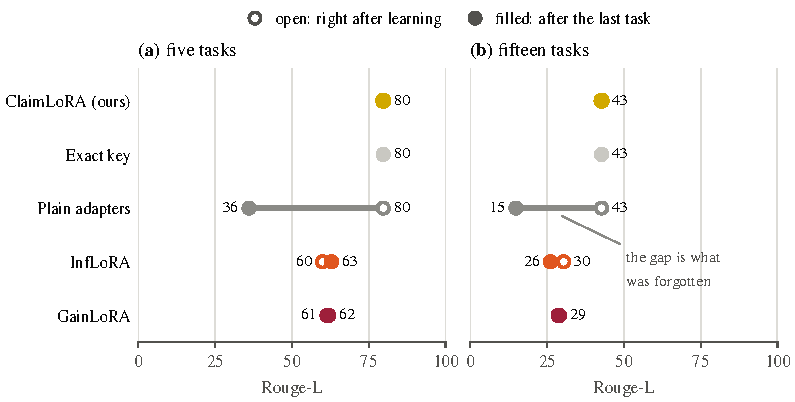
\includegraphics[width=0.9\linewidth]{figures/learn_forget}
  \caption{Learning and forgetting side by side, (a) on five tasks (mean over three seeds) and (b)
  on fifteen tasks (one seed). Open circle: average score of each task right
  after it was learned. Filled circle: average score after the last task. A gap between the two circles
  of a method is forgetting; an open circle far to the left is a lack of learning.}
  \label{fig:learnforget}
\end{figure}

Plain adapters learn and then forget (high open circle, low filled circle). On five tasks the two published methods have low and nearly equal circles: they forget little but learned less within ten epochs, so the comparison does not show that they forget, and we do not claim it. On fifteen tasks their open circles are low as well and the filled circles are lower for InfLoRA and, by less, for GainLoRA: some forgetting and a larger lack of learning, for reasons we did not separate (the method, the short budget, or our set-up). The certified switch has the open circle of plain adapters and no gap, since it leaves the training of an adapter untouched. The published results of both methods used 100 epochs and T5-large; we could not run that setting and the gap in learning may well close there. Without instructions the same two methods did forget more (Section~\ref{sec:nodefpublished}), with the same caveat on learning.

\subsection{What the zones add: a later task that looks like an old one}
\label{sec:stress}

On the benchmark sequences \nearest{} and \cert{} give the same routes, so they cannot show what the frozen zones and the priority of older tasks are for. They matter when a later task resembles an earlier one. A sixth task is added after the five tasks, with inputs of the same
kind as task~2 (SST-2 sentences) and a definition that is one of the rewordings of task~2's definition, as when someone adds ``the same task again'' with a different
instruction. Routes only, one constructed case. Table~\ref{tab:stress} counts how many of the
100 old test inputs of task~2 under each wording are routed differently afterwards.

\begin{table}[t]
  \caption{Stress test (T5-base word-vectors). A sixth task with SST-2 inputs and a
  reworded SST-2 definition is added after the five tasks. ``Blocked'': training
  inputs of the new task inside an older zone, reported when the task arrives. ``Routes
  changed'': old test inputs of task~2 (100 per wording) given to a different task
  afterwards.}
  \label{tab:stress}
  \centering
  \small
  \setlength{\tabcolsep}{4pt}
  \begin{tabular}{lccccccccc}
    \toprule
    & & \multicolumn{4}{c}{Routes changed, \cert{} $\downarrow$} & \multicolumn{4}{c}{Routes changed, \nearest{} $\downarrow$} \\
    \cmidrule(lr){3-6} \cmidrule(lr){7-10}
    New task's definition & Blocked & original & light & medium & heavy & original & light & medium & heavy \\
    \midrule
    light & 799 of 800 & 0 & 0 & 0 & 0 & 0 & 100 & 0 & 0 \\
    medium & 0 of 800 & 0 & 0 & 100 & 2 & 0 & 0 & 100 & 2 \\
    heavy & 0 of 800 & 0 & 0 & 0 & 100 & 0 & 0 & 0 & 100 \\
    \bottomrule
\end{tabular}

\end{table}

\paragraph{A look-alike inside an old zone is blocked and reported.} With the light rewording the inputs of the new task fall inside the zone of task~2: 799 of
its 800 training inputs are blocked, and the user is told when the task arrives, before any
training. Under \cert{} no old input changes its route. Under \nearest{} the old light-wording inputs carry the
instruction of the new task word for word and lie on its signature, so all 100 are
re-routed to it; the same text gets a different answer from then on, and nothing announces it. This is what the frozen zones are for: under the oldest-claim rule a certified input cannot be re-routed by a later task. Whether the old or the new task ought to answer such a text the rules do not
settle. Among \WidenTasksEval{} real tasks with machine-paraphrased instructions this was rare, and the zones did not prevent it there (Sections~\ref{sec:many}, \ref{sec:paraphrase}), so this constructed case is not typical of that collection.

\paragraph{A look-alike outside every zone can take uncertified inputs.} With the medium or heavy rewording the new signature lies outside the zone of task~2, nothing is
blocked, and under both rules the old inputs that carry exactly
that rewording are re-routed (100 of 100, plus 2 heavy-wording inputs in the medium case).
They were never certified; the certified inputs of task~2 (original and light wording) keep their route in every case. The guarantee protects exactly the certified inputs.

\subsection{What the zones cost: 875 real tasks}
\label{sec:many}

A large collection of real tasks contains look-alikes by itself. The \ManyTasks{} tasks of the default English split of Super-NaturalInstructions
\citep{wang2022superni} arrive in a random order, each with its definition and its first inputs (\ManyInputs{} inputs;
openings of \ManyOpeningMin{} to \ManyOpeningMax{} tokens, \ManyOpeningMedian{} in the middle; \ManyOpeningMax{} is the truncation length, so for these tasks the instance is cut off), and each gets its zone when it arrives. Routes only. The rules, including what would count against the method, were fixed
before the run (Appendix~\ref{app:many}).

\begin{table}[t]
  \caption{The zones on \ManyTasks{} real tasks in a random order (T5-base
  word-vectors, unedited instructions). ``Blocked'': inputs of a new task inside an older
  zone when it arrives; the columns count the tasks for which this holds for none, some or all
  of their inputs. ``Routes changed later'': inputs given to a different task
  than right after their own task arrived, under \cert{} / \exactfirst{} / \nearest{}.}
  \label{tab:many}
  \centering
  \small
  \setlength{\tabcolsep}{4pt}
  \begin{tabular}{rccccccc}
    \toprule
    & \multicolumn{3}{c}{Tasks with blocked inputs} & \multicolumn{3}{c}{Inputs to their own task, \%} & Routes \\
    \cmidrule(lr){2-4} \cmidrule(lr){5-7}
    Tasks & none & some & all & \cert{} & \exactfirst{} & \nearest{} & changed later \\
    \midrule
    50 & 49 & 1 & 0 & 98.7 & 100.0 & 100.0 & 0 / 0 / 0 \\
    100 & 96 & 3 & 1 & 96.7 & 100.0 & 100.0 & 0 / 0 / 0 \\
    200 & 178 & 7 & 15 & 90.4 & 99.0 & 98.5 & 0 / 0 / 0 \\
    400 & 337 & 13 & 50 & 85.7 & 99.2 & 99.0 & 0 / 0 / 0 \\
    875 & 724 & 22 & 129 & 83.8 & 98.4 & 98.3 & 0 / 0 / 0 \\
    \bottomrule
\end{tabular}

\end{table}

\begin{figure}[t]
  \centering
  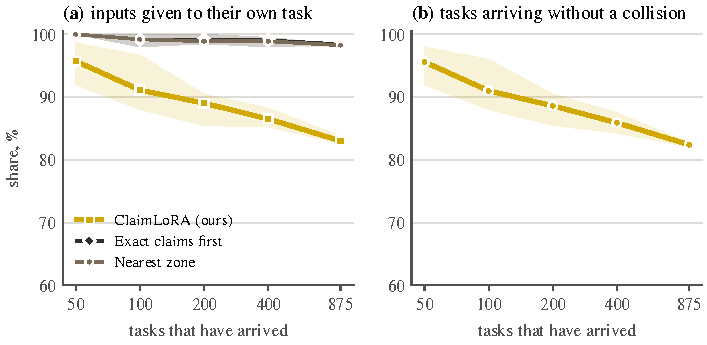
\includegraphics[width=0.86\linewidth]{figures/many}
  \caption{The price of the guarantee as the collection grows (same test as
  Table~\ref{tab:many}; means over five random orders, bands span the lowest
  and the highest). (a) Share of inputs given to their own task; the variant of
  Section~\ref{sec:exactfirst} and the nearest-zone rule nearly coincide. (b) Share of tasks that
  arrive with no input inside an older zone.}
  \label{fig:many}
\end{figure}

\paragraph{The guarantee holds, and its price grows with the collection.} No certified input changed
its route, in any order or at any size. But the larger the
collection, the more often a new task arrives inside an older zone (Figure~\ref{fig:many}). At the end \ManyColliding{} tasks
(\ManyCollidingPct{}\%) have collided with an older task, and for \ManyAllHeld{} every input is
blocked, so that under their given instruction they could not be learned. In four other
random orders \ManyCollidingPctLow{}\% to \ManyCollidingPctHigh{}\% collide,
and \ManyNumericCollidingPct{}\% in the order of the task numbers. These are not
accidents of the geometry: of the \ManyColliding{} colliding tasks, \ManySameText{} have the same
definition text as the task they collide with, \ManyAlikeHigh{} more share at least 80\% of its words,
and none shares less than \ManyAlikeLowest{}\%. They come from families
of tasks whose definitions differ in a word or two: \ManyFamilyMmlu{} are subject variants of one
multiple-choice task and \ManyFamilyAtomic{} relation variants of one classification task
(Table~\ref{tab:manyexamples}).

\paragraph{On unedited instructions the nearest-zone rule is the better rule.} \nearest{} gives
\ManyNearRightPct{}\% of the inputs to their own task and \cert{} \ManyCertRightPct{}\%, and neither re-routes an input later: an
input with an unedited instruction lies exactly on its task's signature, so no other zone can
be nearer. We had written down beforehand that \nearest{}
would re-route inputs here; that was wrong. The weakness of \nearest{} needs edited inputs (Section~\ref{sec:stress}).

\paragraph{The trade.} A zone protects a neighbourhood of an old instruction, where its light rewordings and fewer than half of its machine paraphrases lie, and takes it away from later tasks. Frozen zones block a later sibling and report the collision; a best-match rule serves the sibling and may re-route reworded inputs of the old task. With machine paraphrases of \WidenTasksEval{} real tasks (Section~\ref{sec:paraphrase}) the latter was rare and the zones did not reduce it:
\nearest{} changed \RerouteNearChanged{}\% of the routes (\RerouteNearNChanged{} of \RerouteInputs{}), the same \RerouteCertNChanged{} inputs as \cert{}; the plain nearest signature changed \RerouteSigChanged{}\% and gave more paraphrased inputs to their own task (\RerouteSigOwnEnd{}\% against \RerouteCertOwnEnd{}\%). Which event is more common depends on where a system is used; in a collection built from task
families, as this one is, it is the sibling. The radius factor moves the trade: with
$\kappa = 0.3$, \ManyCleanKappaThree{} of the \ManyTasks{} tasks arrive without a collision
instead of \ManyClean{} (Table~\ref{tab:manykappa}), but only 59\% of the lightly
reworded inputs of the five tasks are certified instead of all (Table~\ref{tab:kappa}). We
kept $\kappa = 0.5$, as fixed before this test.

\paragraph{A variant that serves the siblings.} \exactfirst{} (Section~\ref{sec:exactfirst}) was designed in response to this result, so its numbers on the same
collection are not an independent test. \ExactTasksOwn{} of the \ManyTasks{} tasks receive
all their own inputs when they arrive; the other \ExactTasksNone{} open token for token like an older
task. Nearly all inputs go to their own task in every order (\ExactRightPct{}\% at the end)
and none changes its route later (Table~\ref{tab:many}). In the stress test it serves the look-alike task, \ExactStressOwn{} of its
\StressTrain{} training inputs instead of \CertStressOwn{}, and pays as
Proposition~\ref{prop:exactfirst} says: the 100 old inputs that carry the look-alike's instruction
word for word are handed to it, and no other old input moves. Its routes are almost those of \nearest{}; what differs is what can be promised about an edited input
(Table~\ref{tab:guarantees}). No test separates the two on real inputs (on the French and German machine paraphrases they gave the same routes; on the Spanish ones \nearest{} gives \RerouteNearEsOwn{}\% and the variant \RerouteExactEsOwn{}\% to their own task), and the
variant has not been run with trained answers on a GPU.

\subsection{Mechanical edits of the instruction}
\label{sec:edits}

The instruction is damaged mechanically and the routes are looked at. Every test input of the fifteen tasks (1{,}197 inputs) gets
its own random edit of the task definition: $k$ words of at least four letters with a typo ($k$ capped at the number of such words; two neighbouring inner letters
swapped), $k$ words deleted, or $k$ words replaced by random words from the fifteen
definitions, for $k \in \{1, 2, 4, 8, 16\}$; the definition in lower case; the sentence ``Please
help me with this task.'' in front; the first or the last sentence of the
definition removed; or its sentences shuffled. That makes 23{,}640 edited inputs, routes only. The rules, including the outcomes that would count
against the method, were written into the repository before the run and nothing was changed
afterwards (Appendix~\ref{app:edits}). Line fixed before the run: a
share of inputs on their own task under 80\% for any edit counts against the method.

\begin{figure}[t]
  \centering
  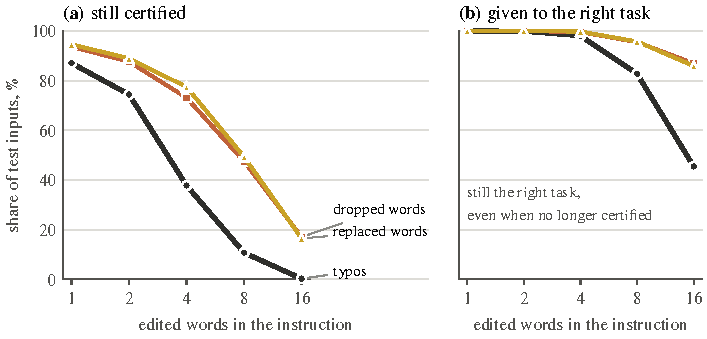
\includegraphics[width=0.86\linewidth]{figures/edits}
  \caption{Mechanical edits of the instruction, all fifteen tasks, routes only (1{,}197 test inputs per point, each with its own random edit). (a) Share of inputs
  still inside their own zone. (b) Share given to their own task.
  No edited input was inside the zone of another task.}
  \label{fig:edits}
\end{figure}

\begin{table}[t]
  \caption{Edits of the whole instruction (same test as Figure~\ref{fig:edits}). Tasks whose
  definition has a single sentence are left out of the last three rows.}
  \label{tab:edits}
  \centering
  \small
  \begin{tabular}{lccccc}
    \toprule
    Edit of the instruction & Tasks & Inputs & Certified inputs, \% & \shortstack[c]{Sent to own\\task, \% $\uparrow$} & Wrong zone \\
    \midrule
    Lower case & 15 & 1197 & 91.4 & 100.0 & 0 \\
    Sentence in front & 15 & 1197 & 91.6 & 100.0 & 0 \\
    First sentence removed & 14 & 1097 & 24.7 & 100.0 & 0 \\
    Last sentence removed & 14 & 1097 & 32.8 & 81.5 & 0 \\
    Sentences shuffled & 14 & 1097 & 100.0 & 100.0 & 0 \\
    \bottomrule
\end{tabular}

\end{table}

\paragraph{No edited input was certified for another task.} Not one of the 23{,}640 edited inputs
lay inside another task's zone; each was certified for its own task or not at all. This holds for these fifteen tasks, whose instructions are far apart; in the collection of Section~\ref{sec:many} inputs of sibling tasks do lie inside older
zones. A certificate promises that an answer stays the same, not that it comes from the right
task.

\paragraph{Small edits keep the certificate, large ones lose it.} With one typo 87.1\% of the inputs
are still certified, with one replaced word 94.6\%, with four edited words 38\% to 77\%, with sixteen
at most 17\% (Figure~\ref{fig:edits}a, Table~\ref{tab:edits}). A typo costs more than a dropped word (93.7\%), presumably because a misspelt word falls apart into
several rare word pieces, which carry a high weight in Eq.~\eqref{eq:weights}.

\paragraph{Heavy damage breaks the route of uncertified inputs.} Up to four edited
words at least 98.1\% of the inputs still reach their own task; with eight typos 82.7\%, with
sixteen typos 45.4\% (Figure~\ref{fig:edits}b). Verdict: the line is crossed, so under badly damaged instructions the nearest-zone route cannot be relied on. What the method offers is the missing certificate, which marks every one of these inputs.

\paragraph{Long instructions are robust, short ones are not.} Tasks whose opening has at least 90 tokens keep
98\% to 100\% of their inputs on the right task even with sixteen typos (Table~\ref{tab:editspertask}). The two tasks that fail
first have the shortest instructions: \texttt{sciq} (ten words, opening of 26
tokens) and \texttt{xsum} (34 tokens); with eight typos only 3\% and 18\% of their inputs arrive. With sixteen typos every word of four or more letters in a definition of ten words carries a typo.

\paragraph{Two findings that follow from how the switch reads.} Removing the last sentence of the
definition leaves 81.5\% of the inputs on their task, but only 2\% for SST-2 and 8\% for emotion
classification, where that sentence states the task. Shuffling the
sentences changes nothing and every input stays certified, because the feature of
Eq.~\eqref{eq:prefix} is an average and ignores word order
(Proposition~\ref{prop:edits}).

\paragraph{The guaranteed tolerance.} The largest distance between two rows of the rescaled
embedding table of T5-base is $D = 509.6$, and the ratio $R_k / D$ of Proposition~\ref{prop:edits}
lies between 2.0\% and 4.2\% for the fifteen tasks. Edits that remove at most this share of the
weight of the opening, and add at most this share, can never leave the zone; in tokens of average weight this is the replacement of \BoundTokensLow{} to \BoundTokensHigh{} tokens,
depending on the task. The measured tolerance is far larger, as it must be, since the bound has to
cover the two most different tokens of the vocabulary. On \BoundInputs{} edited inputs (ten per task and edit with
typos, dropped and replaced words) the bound held for every one: the inputs moved by at most
\BoundWorstPct{}\% of what it allows, \BoundMedianPct{}\% in the middle, and the bound
alone would have certified \BoundGuaranteed{} of the \BoundInside{} inputs that stayed inside
their zone.

\subsection{The order of the tasks}
\label{sec:orders}

The signature of a task depends on its own opening only, and its radius on the signatures known
when it arrives, so the routes under any other order of arrival can be computed exactly without training. Table~\ref{tab:orders} gives them for all
120 orders of the five tasks, the two official orders of the benchmark and 1{,}000 random
orders of the fifteen tasks.

\begin{table}[t]
  \caption{The order of the tasks (routes only, T5-base word-vectors). Entries with four numbers are
  for the original / light / medium / heavy wording; the reworded inputs are those of the five tasks.
  ``Blocked'': training inputs inside an older zone. ``Changed'': test inputs whose route changed
  after their task had been added; a range depends on the order.}
  \label{tab:orders}
  \centering
  \footnotesize
  \setlength{\tabcolsep}{3.5pt}
  \begin{tabular}{lcccccc}
    \toprule
    Sequence & Orders & \shortstack[c]{Sent to own\\task, \% $\uparrow$} & \shortstack[c]{Certified\\inputs, \%} & Wrong zone & Blocked & \shortstack[c]{Routes\\changed $\downarrow$} \\
    \midrule
    5 tasks, all orders & 120 & 100/100/100/93.8 & 100/100/20/19.6 & 0 & 0 & 0--31 \\
    \midrule
    15 tasks, official order 1 & 1 & 100/100/100/93.8 & 100/100/20/19.6 & 0 & 0 & 0 \\
    15 tasks, official order 2 & 1 & 100/100/100/93.8 & 100/100/20/19.6 & 0 & 0 & 31 \\
    15 tasks, random orders & 1,000 & 100/100/100/93.8 & 100/100/20/19.6 & 0 & 0 & 0--31 \\
    \bottomrule
\end{tabular}

\end{table}

In every order all inputs with the original wording are certified, none lies in a foreign
zone, no training input is blocked, and the shares reaching their own task are the
same to the last digit. For 13 of the 15 tasks the nearest known signature is
that of an unrelated task, known from the start, so their radius does not depend on the order (Table~\ref{tab:distances}). The two exceptions are \texttt{samsum} and \texttt{xsum}, whose nearest signature is that of a third summarisation task
(\texttt{reddit\_tifu}); their radius is up to 7\% and 13\% smaller if it was learned
before them, and no test input is affected.

The order decides \emph{when} an uncertified input goes wrong. The 31 heavily
reworded tweets given to SST-2 go to it from the start if SST-2 is learned before
Sentiment140 (our five-task sequence, official order~1). If SST-2 comes later (official
order~2), they first go to their own task and are re-routed when SST-2
arrives: 31 routes change after the inputs were first answered, and with a route the answer
changes in general. They are uncertified, and
Proposition~\ref{prop:uncertified} says this can happen; for certified inputs it cannot.

\subsection{The unrelated inputs}
\label{sec:background}

The collection $\mathcal{B}$ of unrelated inputs sets the token
weights, the scale of distances, and the signatures of the unrelated tasks, which fix most radii. To see whether the results depend on this collection, the route
computations were repeated with two other random draws of the 4{,}000 inputs, with 500, 1{,}000 and 2{,}000 inputs,
and with only five of the ten unrelated tasks in two ways (Table~\ref{tab:background}; the settings and what would count against the method were fixed beforehand, routes only). In
all eight settings every input with the original or the light wording is certified, every input
with the original, light or medium wording reaches its own task, none lies in a foreign zone,
and no training input is blocked: the part of the results that rests on the guarantee did not depend on the choice. The share of heavily reworded inputs that reach their own task did,
from \BackgroundHeavyLow{}\% to \BackgroundHeavyHigh{}\%, so the 93.8\% of the main configuration is one draw from that range and not a property of the method.
We had expected the radii to change with only five unrelated tasks; they hardly did, and at most two more heavily reworded inputs were certified.

\subsection{Other models}
\label{sec:models}

\paragraph{The routes with other embedding tables.} The switch needs only a tokenizer and an embedding table, so the routes can be computed without training for any
model. Table~\ref{tab:models} does this for eight models: T5 in three sizes \citep{raffel2020t5} and Flan-T5
\citep{chung2024flant5}, GPT-2 \citep{radford2019gpt2}, SmolLM2
\citep{allal2025smollm2}, Qwen2.5 \citep{yang2024qwen25} and RoBERTa
\citep{liu2019roberta}, with embedding dimensions from 512 to 1024 and five different
vocabularies. Nothing was adjusted per model; the radius factor and word weights are those of
Section~\ref{sec:method}. Routes only. For every model, every test input with the original wording lies in its
own zone in the five-task and the 15-task sequence, none lies in a foreign zone, and no
training input of a later task is blocked. With light rewording 99\% to 100\% of the inputs are
certified and with medium rewording all reach their own task. Models differ under heavy rewording: 80\% to 99\% reach their own task, and the routes of three uncertified inputs changed when a later task arrived (two with Flan-T5, one with GPT-2); no certified route changed.

\begin{table}[t]
  \caption{Routes computed with the embedding tables of eight models (CPU, no training). Entries
  with four numbers are for the original / light / medium / heavy wording. ``Wrong zone'': inputs
  inside the zone of another task, over both sequences and all wordings. ``Changed'': inputs
  whose route changed after their task had been added. With the original wording every input of
  the 15-task sequence is certified for every model.}
  \label{tab:models}
  \centering
  \footnotesize
  \setlength{\tabcolsep}{3pt}
  \begin{tabular}{lcccccc}
    \toprule
    & & \multicolumn{2}{c}{Five tasks} & Fifteen tasks & & \\
    \cmidrule(lr){3-4} \cmidrule(lr){5-5}
    Embedding table of & \shortstack[c]{Embedding\\dimension\\$d$} & \shortstack[c]{certified\\inputs, \%} & \shortstack[c]{sent to\\own task,\\\% $\uparrow$} & \shortstack[c]{sent to\\own task,\\\% $\uparrow$} & Wrong zone & \shortstack[c]{Routes\\changed\\$\downarrow$} \\
    \midrule
    \texttt{t5-small} & 512 & 100/100/20/20 & 100/100/100/89 & 100/100/100/89 & 0 & 0 \\
    \texttt{t5-base} & 768 & 100/100/20/20 & 100/100/100/94 & 100/100/100/94 & 0 & 0 \\
    \texttt{t5-large} & 1024 & 100/100/20/19 & 100/100/100/83 & 100/100/100/83 & 0 & 0 \\
    \texttt{flan-t5-base} & 768 & 100/100/20/14 & 100/100/100/99 & 100/100/100/99 & 0 & 2 \\
    \texttt{gpt2} & 768 & 100/99/20/20 & 100/100/100/87 & 100/100/100/87 & 0 & 1 \\
    \texttt{SmolLM2-135M} & 576 & 100/99/20/20 & 100/100/100/82 & 100/100/100/82 & 0 & 0 \\
    \texttt{Qwen2.5-0.5B} & 896 & 100/99/20/20 & 100/100/100/80 & 100/100/100/80 & 0 & 0 \\
    \texttt{roberta-base} & 768 & 100/99/20/20 & 100/100/100/94 & 100/100/100/93 & 0 & 0 \\
    \bottomrule
\end{tabular}

\end{table}

\paragraph{Training other models with the stand-alone code.} The stand-alone implementation
(Appendix~\ref{app:impl}) was run on T5-small, GPT-2 and
SmolLM2-135M on a CPU: five tasks, 400 training
examples and five epochs each, 30 to 50 test inputs per task, one seed. The runs are small on purpose: they show whether the code
keeps answers on another architecture, not how good these models can become. In all three (Table~\ref{tab:demo}) the certified switch ends exactly where it stood right after learning, no
answer of an earlier task changes, and every test input with the original wording is certified. With
all adapters on, the same adapters end far lower and nearly all answers of earlier tasks change. With heavily reworded instructions no answer changes either, and
\DemoTfiveHeavyRight{}\%, \DemoGptHeavyRight{}\% and \DemoSmolHeavyRight{}\% of those inputs reach
their own task.

\begin{table}[t]
  \caption{The stand-alone implementation on three small models (CPU, five tasks, 400 training
  examples and 5 epochs per task, one seed). ``Changed'': answers of the first four tasks that
  differ at the end. ``Certified'': test inputs with the original wording inside a zone.
  ``enc.-dec.'': encoder-decoder; ``dec.-only'': decoder-only.}
  \label{tab:demo}
  \centering
  \footnotesize
  \setlength{\tabcolsep}{3pt}
  \begin{tabular}{llcccccccc}
    \toprule
    & & \multicolumn{3}{c}{\cert{}, original} & \multicolumn{2}{c}{\plain{}, original} & & \multicolumn{2}{c}{\cert{}, heavy} \\
    \cmidrule(lr){3-5} \cmidrule(lr){6-7} \cmidrule(lr){9-10}
    Model & Kind & \shortstack[c]{Score\\right\\after\\learning\\$\uparrow$} & \shortstack[c]{Final\\score\\$\uparrow$} & \shortstack[c]{Answers\\changed $\downarrow$} & \shortstack[c]{Final\\score\\$\uparrow$} & \shortstack[c]{Answers\\changed $\downarrow$} & \shortstack[c]{Certified\\inputs} & \shortstack[c]{Final\\score\\$\uparrow$} & \shortstack[c]{Answers\\changed $\downarrow$} \\
    \midrule
    \texttt{SmolLM2-135M} & dec.-only & 74.3 & 74.3 & 0 of 120 & 27.7 & 100 of 120 & 150 of 150 & 65.1 & 0 of 120 \\
    \texttt{gpt2} & dec.-only & 67.9 & 67.9 & 0 of 120 & 15.8 & 119 of 120 & 150 of 150 & 54.8 & 0 of 120 \\
    \texttt{t5-small} & enc.-dec. & 65.8 & 65.8 & 0 of 200 & 12.0 & 200 of 200 & 250 of 250 & 56.2 & 0 of 200 \\
    \bottomrule
\end{tabular}

\end{table}

\paragraph{A sibling task, with trained answers.} \exactfirst{} was also run with the
stand-alone code on T5-small. After the five tasks a sixth is learned: the sentences of SST-2
under the lightly reworded SST-2 definition, with other answer words (``good'' and ``bad''
instead of ``POS'' and ``NEG'') so that one can see which adapters answered, learned
twice from the same starting point. Under \cert{} all \SiblingCertBlocked{} of its
\SiblingTrain{} training inputs are blocked; its test inputs are still answered in
the words of the old task (\SiblingCertRight{} of \SiblingTest{} right), and no answer of the five
old tasks changes in any wording. Under \exactfirst{} the task is learned (\SiblingExactRight{} of
\SiblingTest{} right), no answer to an unedited input of the old tasks changes, and the
\SiblingExactChangedLight{} old SST-2 test inputs that carry the sibling's instruction word for
word now get the sibling's answer; nothing else changes (\SiblingOldInputs{} old test inputs per
wording). This is one small model and one constructed sibling, not a test of the variant at scale.
